\documentclass[a4paper,11pt]{scrartcl}

\usepackage[ngerman]{babel}
\usepackage[T1]{fontenc}
\usepackage[utf8]{inputenc}
\usepackage{times}
\usepackage{graphicx}
\usepackage{apacite}
\usepackage[hyphens]{url}

\begin{document}

\title{Digital Rights Management}
\subtitle{Encrypted Media Extensions}
\author{Patrick Bucher}
\date{\today}
\maketitle

\tableofcontents

\section{DRM: Digital Rights Management}

DRM steht für \textit{Digital Rights Management}. Der Duden definiert DRM als «Gesamtheit der Strategien und Maßnahmen zur Kontrolle der Nutzung digitaler Medien» \cite{duden}. Es geht also um die Verwaltung von Rechten im Zusammenhang mit digitalen Medien. Einem Lizenzeigner sollen bestimmte Nutzungsrechte gewährt werden. Personen ohne eine solche Lizenz sollen von der Nutzung ausgeschlossen werden. Darum steht DRM für Anhänger der «Free Software»-Bewegung auch für \textit{Digital Restriction Management} \cite{defectivebydesign}. Die beiden Begriffe beschreiben das gleiche, einfach aus einer anderen Perspektive.

DRM-Verfahren kommen etwa in folgenden Bereichen zum Einsatz:

\begin{itemize}
    \item{auf digitalen Datenträgern wie CD, DVD und Blu-ray-Disc als Kopierschutzmechanismus}
    \item{auf eBook-Plattformen wie Adobe Digital Editions oder Amazon Kindle zur Verwaltung der Leserechte}
    \item{bei digitalen Schnittstellen wie DVI und HDMI zur Verhinderung unautorisierten Abspielens von Videos}
\end{itemize}

Hier soll es um DRM im Zusammenhang mit dem Abspielen von Videos im Webbrowser gehen, genauer um die \textit{Encrypted Media Extensions}.

\section{EME: Encrypted Media Extensions}

\subsection{Motivation}

Wollte man sich vor einigen Jahren noch ein Video im Browser anschauen, war man auf Plugins wie RealPlayer oder Adobe Flash angewiesen. HTML5 brachte dann das \texttt{<video>}-Element mit, und die Browser implementierten Funktionen zum Abspielen von Videos. Das funktioniert für kostenlose Inhalte mittlerweile hervorragend. Das Problem ist aber, dass kostenpflichtige Angebote wie Netflix und Zattoo ihre Videos nur denjenigen (ohne Einschränkung) zeigen wollen, die vorher dafür bezahlt haben. Das funktioniert mit dem durch HTML5 spezifizierten \texttt{<video>}-Element nicht. Darum setzen kommerzielle Angebote weiterhin auf Technologien wie Microsoft Silverlight und Adobe Flash. Der HTML5-Standard muss also um entsprechende DRM-Mechanismen ergänzt werden, um kostenpflichtige Videoinhalte künftig ganz ohne Browser-Plugins abspielen zu können.

\subsection{Status}

Eine W3C-Arbeitsgruppe spezifizierte die \textit{Encrypted Media Extensions} als optionale Erweiterung für HTML5-Videos \cite{w3c}. Ein Browser, der die EME nicht implementiert, kann somit trotzdem noch standardkonform sein. Die EME beschreiben kein DRM-System, sondern eine API, womit DRM implementiert werden kann \cite{html5rocks}. Die EME sind noch kein etablierter Standard, sondern liegen als \textit{Proposed Recommendation} vor: die zweithöchste Stufe des fünfstufigen W3C-Standardisierungsprozederes. Webbrowser wie Chrome, Firefox, Safari, Edge und Internet Explorer haben die EME bereits teilweise implementiert. Netflix funktioniert auf Chromebooks (die auf Linux basieren und auf denen Silverlight nicht funktioniert) bereits seit 2013 über die EME \cite{netflix}.

\subsection{Komponenten}

Da die EME kein komplettes DRM-System, sondern bloss eine API spezifizieren, werden darin keine Vorgaben über die eingesetzten kryptografischen Mechanismen und Verfahren gemacht. Dies ist Gegenstand einer anderen W3C-Spezifikation, der \textit{Web Cryptography API}, die derzeit als \textit{Recommendation} vorliegt \cite{w3c-crypto}.

Die Schlüssel müssen auf einem \textit{License Server} abgelegt sein, und die \textit{Web Application} (d.h. die Webseite mit den Videos) muss wissen, wo der Schlüssel für welches verschlüsselte Video zu finden ist. Die eigentliche Rechteverwaltung -- wer Zugriff auf welche Videos hat -- ist Sache der \textit{Web Application} bzw. deren Entwickler.

Das Herzstück der EME ist das \textit{Content Decryption Module} (CDM), welches die eigentliche Entschlüsselung (und optional auch die Dekodierung) der Videodatei vornimmt. Es kann als Bestandteil des Browsers implementiert oder als Plugin nachinstallierbar sein -- oder sogar als Hardware oder Firmware umgesetzt werden.

\subsection{Ablauf}

Gelangt der Benutzer auf eine Seite mit einem EME-geschützen Video, passiert folgendes:

\begin{itemize}
    \item{Der \textit{Browser} lädt eine \textit{Web Application} (1a). Diese enthält ein DRM-geschütztes Dokument (die \textit{Encrypted Media}), sprich ein Video (1b).}
    \item{Der \textit{Browser} liest die Metadaten der \textit{Encrypted Media} aus (2a) und stellt fest, dass diese verschlüsselt ist (2b). Darauf löst der \textit{Browser} den \texttt{encrypted}-Event aus, der von der \textit{Web Application} entgegengenommen wird (2c).}
    \item{Die \textit{Web Application} erstellt eine \texttt{MediaKeySession} (3), welche als Container für die Lizenzschlüssel fungiert, und sendet die Metadaten des Videos an das \textit{CDM} (4).}
    \item{Das \textit{CDM} löst einen \texttt{message}-Event aus (5), welcher von der \texttt{MediaKeySession} abgefangen wird. Diese stellt nun über die \textit{Web Application} eine Key-Anfrage an den \textit{License Server} (6).}
    \item{Der \textit{License Server} antwortet und schickt den Lizenzschlüssel an die \textit{Web Application} zurück (7a). Diese aktualisiert die \texttt{MediaKeySession} mit dem neuen Lizenzschlüssel (7b), welcher nun dem \textit{CDM} zur Verfügung steht.}
    \item{Das \textit{CDM} kann nun die \textit{Encrypted Media} entschlüsseln (8a) und im Browser abspielen lassen (8b).}
\end{itemize}

Abbildung \ref{fig:EMEWF} veranschaulicht diesen Prozess.

%\begin{figure}
%   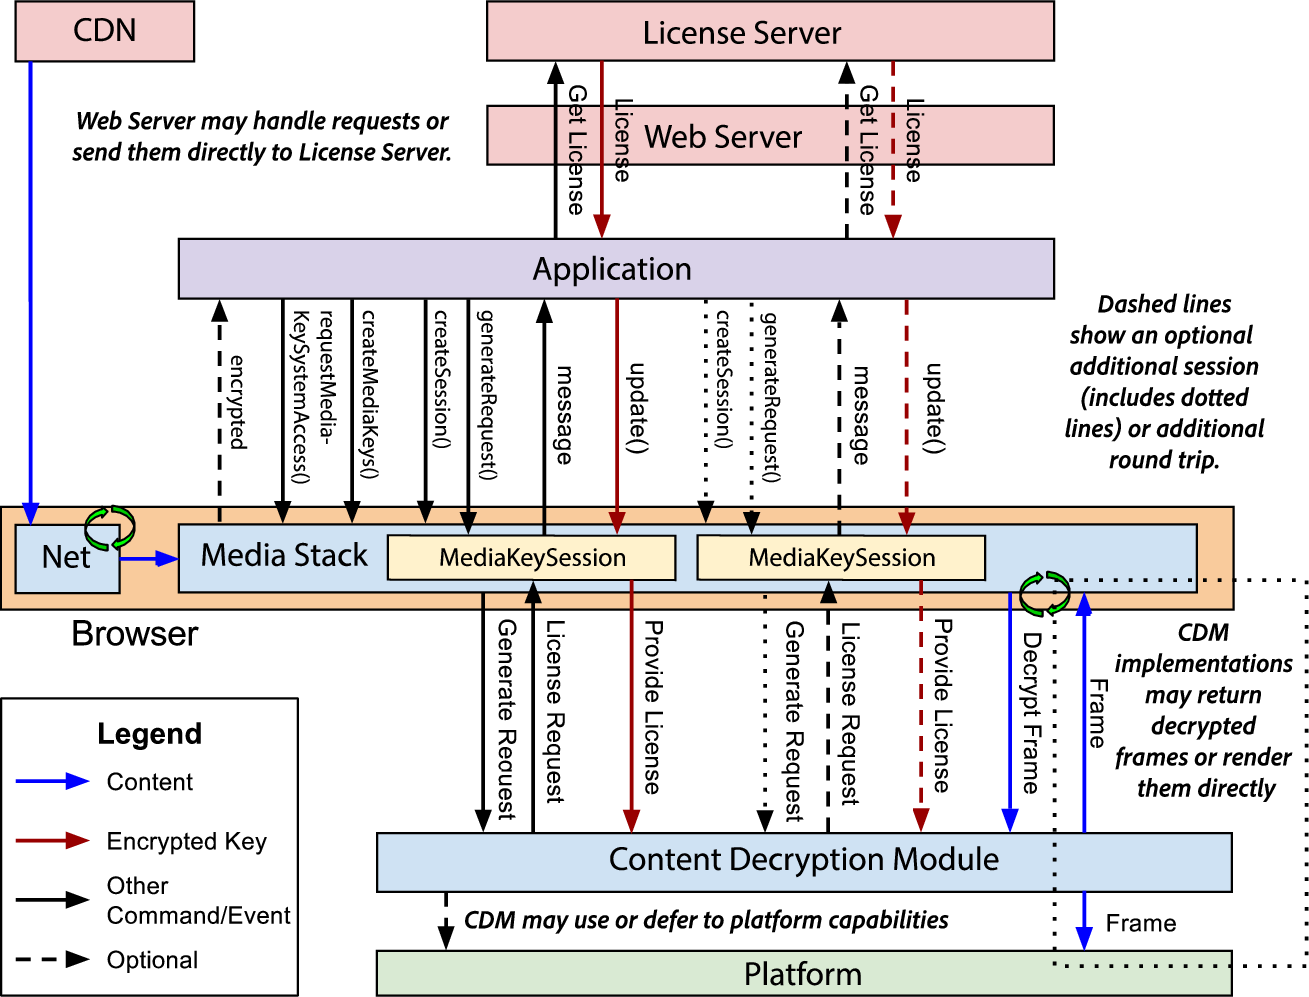
\includegraphics[width=1.0\textwidth]{eme-overview.png}
%   \caption{Der EME-Stack\protect\footnotemark}
%   \label{fig:EME}
%\end{figure}
%\footnotetext{Quelle: \url{https://www.w3.org/TR/encrypted-media/stack-overview.svg}}

\begin{figure}
    %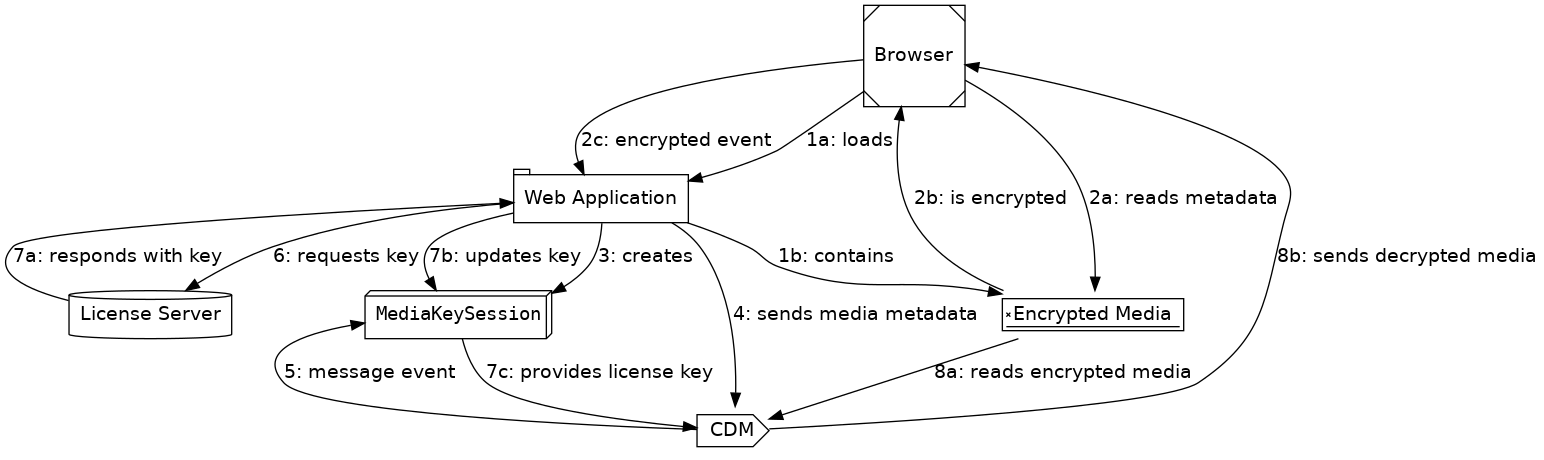
\includegraphics[width=1.0\textwidth]{eme-td.png}
    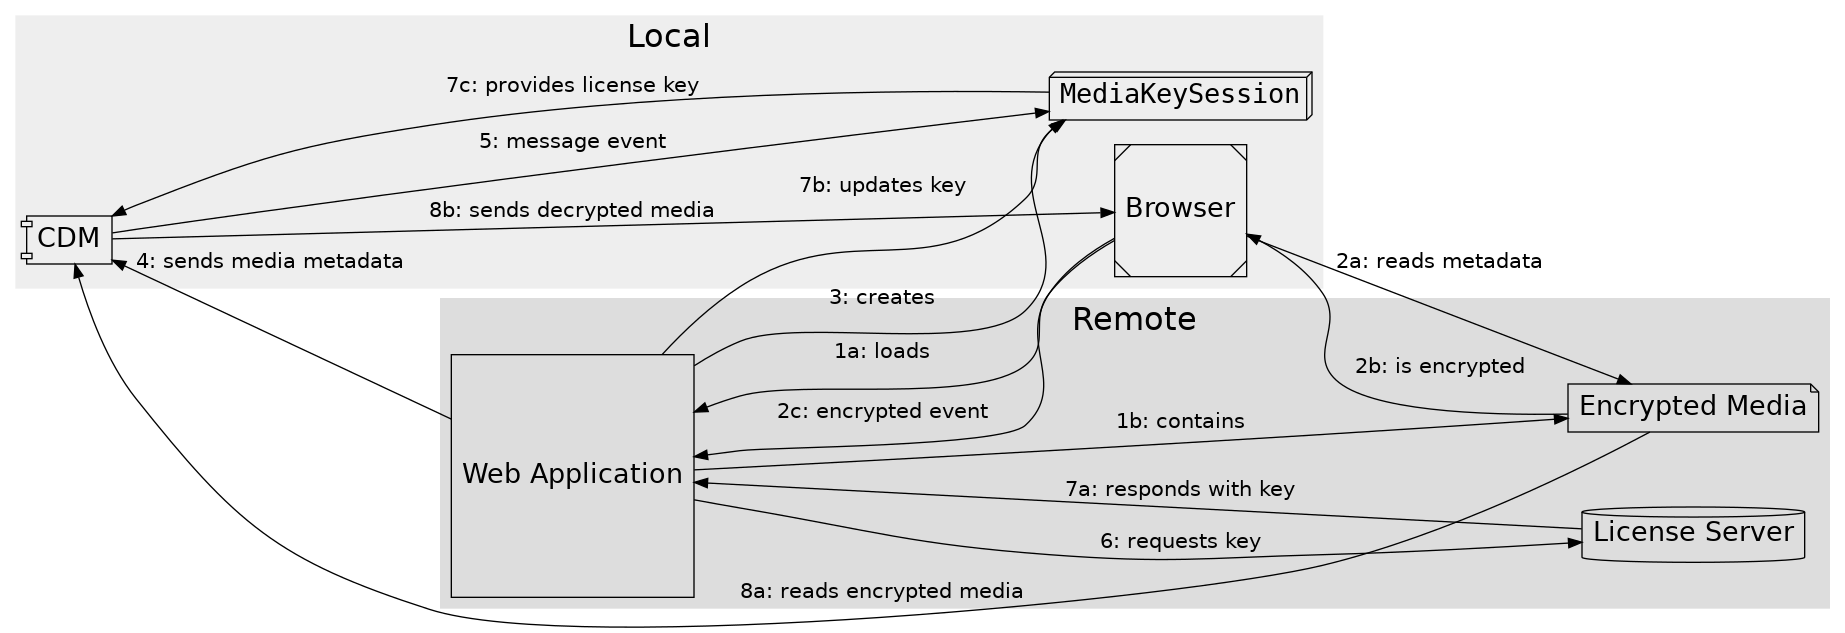
\includegraphics[width=1.0\textwidth]{eme-clustered.png}
    \caption{Das Abspielen eines EME-geschützten Videos}
    \label{fig:EMEWF}
\end{figure}

\subsection{Fallbeispiel: Netflix 4k-Videos}

Seit Ende 2016 bietet Netflix vereinzelte Filme und Serien in 4k-Auflösung (ca. 4000$\times$2000 Bildpunkte) an \cite{netflix-4k}. Um in den Genuss solch hochauflösender Videos zu kommen benötigt man aber mehr als einen 4k-Monitor, eine schnelle Internetverbindung und ein Netflix-Abo: Die 4k-Auflösung funktioniert nur auf Intel-Rechnern der neuesten Generation («Kaby Lake»). Angeblich seien nur diese Chips schnell genug, um \textit{HEVC}-codierte (\textit{High Efficiency Video Codec}, auch als \textit{h265} bekannt) 4k-Videos in Echtzeit zu dekodieren.

Die Begründung wirkt fadenscheinig, zumal Konkurrenzprodukte wie Radeon RX400 und GeForce GTX 1000 die zum Dekodieren erforderliche Performance problemlos erreichen. Tatsächlich dürfte ein noch nicht implementierter Kopierschutzmechanismus in den entsprechenden Treibern ausschlaggebend sein \cite{heise}. Die 4k-Auflösung steht nur dann zur Verfügung, wenn man Netflix über den Webbrowser Edge von Microsoft oder über die passende Windows-App verwendet \cite{pcworld}. Diese Einschränkung hat nichts mit der Hardware-Performance zu tun, vielmehr haben Microsoft und Netflix ein CDM ausgearbeitet, das sie anderen Anbietern nur eingeschränkt zur Verfügung stellen. Mitgliedern des \textit{Windows Insider Programs} steht mittlerweile ein experimenteller Treiber für GeForce-Grafikkarten zur Verfügung, womit sich die 4k-Videos von Netflix abspielen lassen sollen \cite{nvidia}. Linux-Anwender werden noch länger auf die Serie \textit{Gilmore Girls} in 4k-Auflösung verzichten müssen.

Das CDM scheint also aus einer Software- (Browser, App) und einer Hardware- bzw. Treiber-Komponente zu bestehen. Weder von Netflix noch von den Grafikkartenherstellern lassen sich genauere Informationen darüber in Erfahrung bringen. Dass die 4k-Auflösung bisher nur mit Software von Microsoft zur Verfügung steht, deutet auf die Verwendung von \textit{PlayReady 3.0} -- einem DRM-Verfahren aus dem Hause Microsoft -- hin, das bereits in Intel- und (experimentell) Nvidia-GeForce-Grafiktreibern implementiert ist, jedoch noch nicht in den Radeon-Grafiktreibern von AMD.


\subsection{Kritik}

Das CDM umfasst je nach Hersteller und Implementierung andere Funktionalitäten. Wie das Netflix-4k-Beispiel zeigt, können sich Videostreaming-Plattformen mit Browser- und Hardware-Herstellern absprechen und ihre CDM nur noch für bestimmte Plattformen freigeben. Solche Absprachen könnten zu einem handfesten Marktvorteil führen, wobei in diesem Beispiel Microsoft zuungunsten von Apple (Mac OS, Safari), Google (Chrome) und Mozilla (Firefox) -- bzw. Intel zuungunsten von AMD und Nvidia profitiert. Das offen konzipierte und auf Standards basierende Web könnte so bald von einzelnen Herstellern kontrolliert werden, zumindest was das Videostreaming anbelangt.

Ein CDM kann nicht nur zum Entschlüsseln, sondern auch zum Dekodieren von Videos verwendet werden. So könnten neue, hoch leistungsfähige Videocodecs nur den Benutzern zur Verfügung gestellt werden, die bereit sind ein proprietäres CDM zu installieren. Damit könnten Anbieter geschützter Videos Druck auf die Anwender ausüben. Glücklicherweise scheinen sich die meisten Anbieter von Videoplattformen (Netflix, Amazon), Webbrowsern (Microsoft, Firefox, Google) und Hardware (Intel, Nvidia, AMD) auf einen offenen und gebührenfreien Video-Codec einigen zu können \cite{aomedia}. Einzig Apple, das mit eigener Hardware, einem eigenen Betriebssystem, einem eigenen Browser und eigenen Vertriebskanälen ein geschlossenes «Ökosystem» bildet, könnte zum Spielverderber werden.

Viele Anbieter werden ihre CDM als Binärmodule und nicht quelloffen (mit entsprechender Open-Source-Lizenz) zur Verfügung stellen. Das ist gerade bei den Open-Source-Browsern Chrome und Firefox ein Problem. Für Firefox soll dieses Problem entschärft werden, indem das CDM als Plugin nachgeladen und nicht direkt im Browser implementiert wird.

Für Sicherheitsforscher stellen CDM ein gewaltiges Problem dar, da das Reverse-Engineering dieser Komponenten unter den \textit{Digital Millenium Copyright Act} fällt (\textit{DMCA}; Umgehung von Kopierschutzmechanismen) und somit verboten ist.

Wer sich in Zukunft kostenpflichtige Videos im Webbrowser anschauen will, der wird sich vorerst zwischen den proprietären Lösungen Adobe Flash und Microsoft Silverlight einerseits und den proprietären EME-Browsermodulen (mit entsprechender Grafikkarte und Software) andererseits entscheiden müssen. Der Einwand, dass wer sich proprietäre Videos anschauen will auch proprietäre Software ausführen soll, greift zu kurz, zumal die EME-Spezifikation der Grundidee des «freien» Webs zuwiderläuft. 

\bibliography{paper.bib}
\bibliographystyle{apacite}

\end{document}
